\documentclass[]{article}
\usepackage{graphicx}
\usepackage{subfigure}

%opening
\title{Pub Website Development}
\author{John Alton}

\begin{document}

\maketitle

\begin{abstract}
	This document is designed to plan and document the development process from design through to implementation and testing.
\end{abstract}

\section{Specification}
The main purpose if this project is to create a web based solution which will keep track of rounds bought at the pub. Firstly it is the most important feature that \textbf{each individuals `balance' can be determined}, this refers to the amount of money they have spent on drinks relative to the amount of money that has been spent on them by other people. Several side features however include the ability to look back at recent rounds, including who attended, what each person drank and when the round took place. A further side task is that it should be able to determine the order of people who have the lowest balance since they will be next to buy drinks. In order for this to work it will also be necessary to add new `people' and `drinks'.

\section{Design}
\subsection{Overview}
I believe the best package for this development is that of a website, primarily because it is then easy for everybody to access but also because it will provide valuable experience in web development. I believe the necessary skills for this will include HTML, CSS, JavaScript, PHP and SQL. 

First it will be necessary to design the interface, this will need to be created using a combination of HTML and CSS. However I will design the interface using GIMP image editor prior to the development. Separate to this I will also create a storyboard which should show how specific features on each page behave, it should also show the links between the various pages. From here I will design the database which is to be implemented on the server side in order to store the necessary information. Once the design phase is complete I will proceed to the implementation phase. First by creating the HTML and CSS which will replicate the interface that has been designed, then I will proceed to implement the database along with any necessary SQL statements used for gathering the necessary information.  

\subsection{Interface}
The interface should be as simple as possible, primarily graphical, keeping the text to a minimum. It is not intended for users with technical knowledge and should be kept simple. The only screens that it needs to be designed for are PC/Laptop, it will not be necessary to make this accessible from mobile devices. 

First I had a look at several website designs in order to find inspiration. I believe that a very clean interface would be 

\begin{figure*}[t!]
	\centering
	\begin{subfigure}
		\centering
		
\includegraphics[height=1.2in]{Images/idea1}
		\caption{Lorem ipsum}
	\end{subfigure}%
	~ 
	\begin{subfigure}
		\centering
		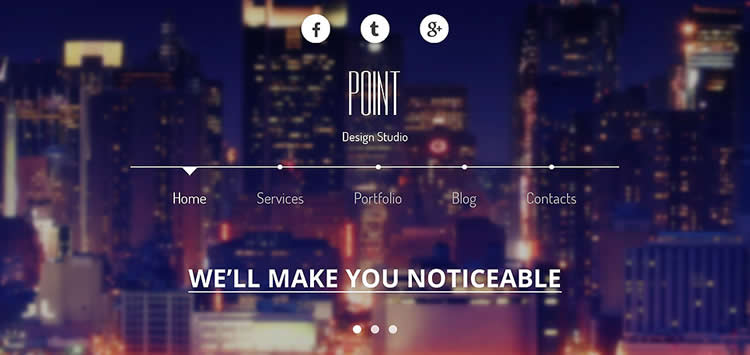
\includegraphics[height=1.2in]{Images/idea2}
		\caption{Lorem ipsum, lorem ipsum,Lorem ipsum, lorem ipsum,Lorem ipsum}
	\end{subfigure}
	\caption{Caption place holder}
\end{figure*}

\end{document}
